\documentclass{standalone}
\usepackage{tikz}
\usetikzlibrary{patterns, positioning}


\begin{document}
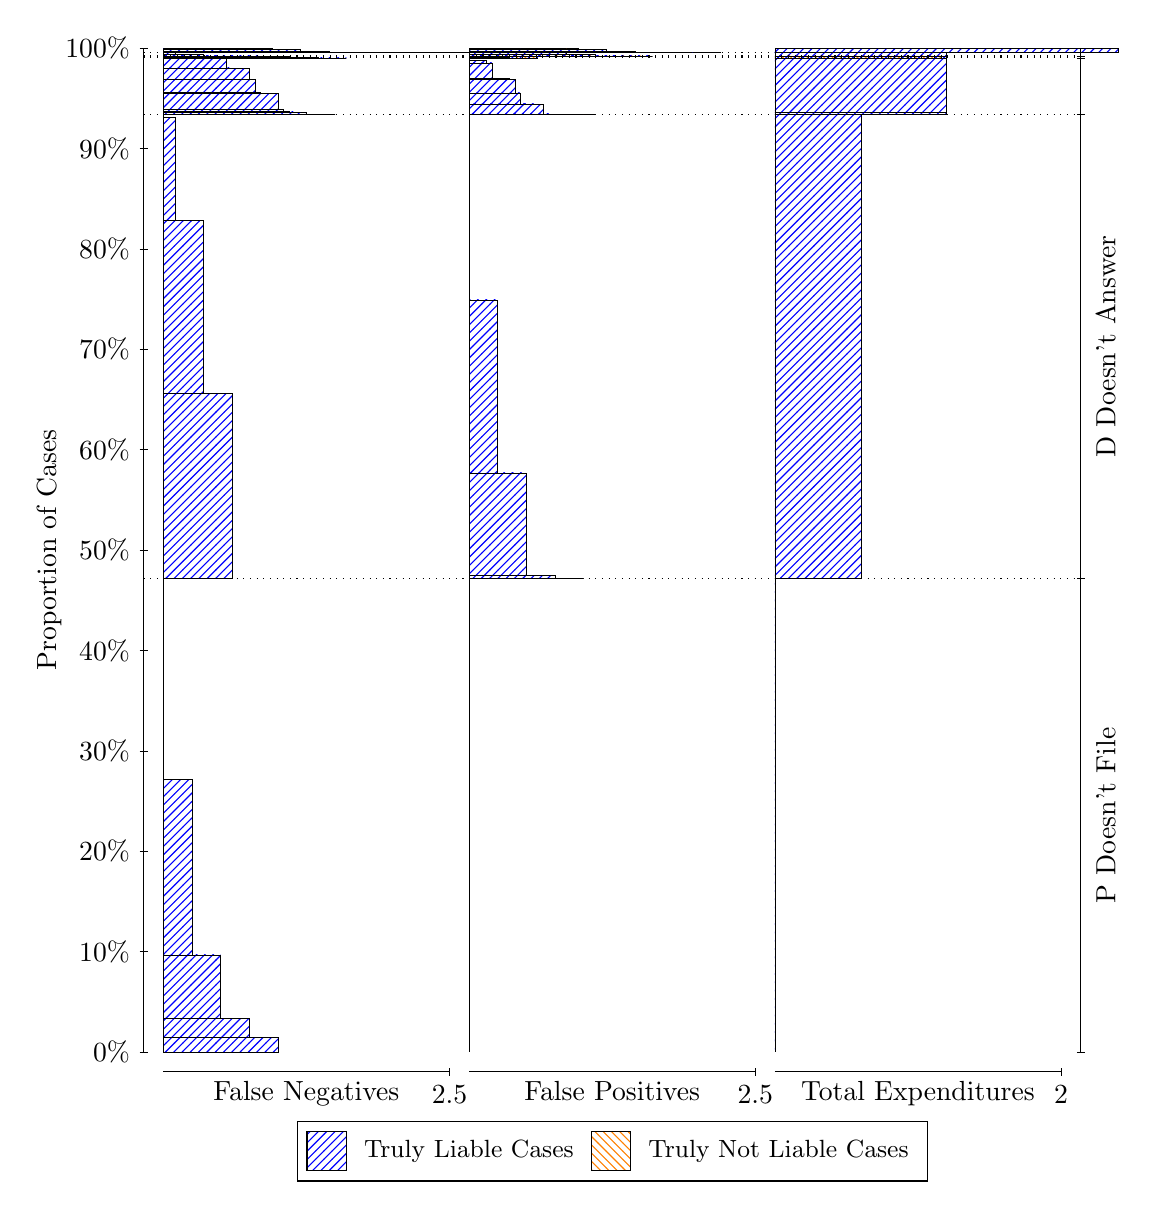
\begin{tikzpicture}
\draw[black, very thin] (1.5,1.75) -- (1.5,14.5);
\node[rotate=90, text=black, anchor=center] at (0.3, 8.125) {Proportion of Cases};
\draw[black, very thin] (1.45,1.75) -- (1.55,1.75);
\node[text=black, anchor=east] at (1.45, 1.75) {0\%};
\draw[black, very thin] (1.45,3.025) -- (1.55,3.025);
\node[text=black, anchor=east] at (1.45, 3.025) {10\%};
\draw[black, very thin] (1.45,4.3) -- (1.55,4.3);
\node[text=black, anchor=east] at (1.45, 4.3) {20\%};
\draw[black, very thin] (1.45,5.575) -- (1.55,5.575);
\node[text=black, anchor=east] at (1.45, 5.575) {30\%};
\draw[black, very thin] (1.45,6.85) -- (1.55,6.85);
\node[text=black, anchor=east] at (1.45, 6.85) {40\%};
\draw[black, very thin] (1.45,8.125) -- (1.55,8.125);
\node[text=black, anchor=east] at (1.45, 8.125) {50\%};
\draw[black, very thin] (1.45,9.4) -- (1.55,9.4);
\node[text=black, anchor=east] at (1.45, 9.4) {60\%};
\draw[black, very thin] (1.45,10.675) -- (1.55,10.675);
\node[text=black, anchor=east] at (1.45, 10.675) {70\%};
\draw[black, very thin] (1.45,11.95) -- (1.55,11.95);
\node[text=black, anchor=east] at (1.45, 11.95) {80\%};
\draw[black, very thin] (1.45,13.225) -- (1.55,13.225);
\node[text=black, anchor=east] at (1.45, 13.225) {90\%};
\draw[black, very thin] (1.45,14.5) -- (1.55,14.5);
\node[text=black, anchor=east] at (1.45, 14.5) {100\%};

\draw[black, very thin] (13.4,1.75) -- (13.4,14.5);
\draw[black, very thin] (13.35,1.75) -- (13.45,1.75);
\node[anchor=west] at (13.35, 1.75) {};
\draw[black, very thin] (13.35,7.76) -- (13.45,7.76);
\node[anchor=west] at (13.35, 7.76) {};
\draw[black, very thin] (13.35,13.661) -- (13.45,13.661);
\node[anchor=west] at (13.35, 13.661) {};
\draw[black, very thin] (13.35,14.375) -- (13.45,14.375);
\node[anchor=west] at (13.35, 14.375) {};
\draw[black, very thin] (13.35,14.399) -- (13.45,14.399);
\node[anchor=west] at (13.35, 14.399) {};
\draw[black, very thin] (13.35,14.442) -- (13.45,14.442);
\node[anchor=west] at (13.35, 14.442) {};
\draw[black, very thin] (13.35,14.5) -- (13.45,14.5);
\node[anchor=west] at (13.35, 14.5) {};

\draw[black, very thin, pattern color=blue, pattern=north east lines] (1.75,1.75) rectangle (3.2033,1.9327);
\draw[black, very thin, pattern color=blue, pattern=north east lines] (1.75,1.9327) rectangle (2.84,2.1754);
\draw[black, very thin, pattern color=blue, pattern=north east lines] (1.75,2.1754) rectangle (2.4767,2.982);
\draw[black, very thin, pattern color=blue, pattern=north east lines] (1.75,2.982) rectangle (2.1133,5.2132);
\draw[black, very thin, pattern color=orange, pattern=north west lines] (1.75,5.2132) rectangle (1.75,5.2132);
\draw[black, very thin, pattern color=blue, pattern=north east lines] (1.75,5.2132) rectangle (1.75,7.76);
\draw[black, very thin, pattern color=blue, pattern=north east lines] (1.75,7.76) rectangle (2.622,10.118);
\draw[black, very thin, pattern color=blue, pattern=north east lines] (1.75,10.118) rectangle (2.2587,12.315);
\draw[black, very thin, pattern color=blue, pattern=north east lines] (1.75,12.315) rectangle (1.8953,13.615);
\draw[black, very thin, pattern color=orange, pattern=north west lines] (1.75,13.615) rectangle (1.75,13.615);
\draw[black, very thin, pattern color=blue, pattern=north east lines] (1.75,13.615) rectangle (1.75,13.661);
\draw[black, very thin, pattern color=blue, pattern=north east lines] (1.75,13.661) rectangle (3.93,13.661);
\draw[black, very thin, pattern color=blue, pattern=north east lines] (1.75,13.661) rectangle (3.7847,13.661);
\draw[black, very thin, pattern color=blue, pattern=north east lines] (1.75,13.661) rectangle (3.6393,13.662);
\draw[black, very thin, pattern color=blue, pattern=north east lines] (1.75,13.662) rectangle (3.5667,13.686);
\draw[black, very thin, pattern color=blue, pattern=north east lines] (1.75,13.686) rectangle (3.494,13.686);
\draw[black, very thin, pattern color=blue, pattern=north east lines] (1.75,13.686) rectangle (3.4213,13.688);
\draw[black, very thin, pattern color=blue, pattern=north east lines] (1.75,13.688) rectangle (3.3487,13.695);
\draw[black, very thin, pattern color=blue, pattern=north east lines] (1.75,13.695) rectangle (3.276,13.723);
\draw[black, very thin, pattern color=blue, pattern=north east lines] (1.75,13.723) rectangle (3.2033,13.92);
\draw[black, very thin, pattern color=blue, pattern=north east lines] (1.75,13.92) rectangle (3.1307,13.922);
\draw[black, very thin, pattern color=blue, pattern=north east lines] (1.75,13.922) rectangle (3.058,13.924);
\draw[black, very thin, pattern color=blue, pattern=north east lines] (1.75,13.924) rectangle (2.9853,13.937);
\draw[black, very thin, pattern color=blue, pattern=north east lines] (1.75,13.937) rectangle (2.9127,14.104);
\draw[black, very thin, pattern color=blue, pattern=north east lines] (1.75,14.104) rectangle (2.84,14.246);
\draw[black, very thin, pattern color=blue, pattern=north east lines] (1.75,14.246) rectangle (2.7673,14.246);
\draw[black, very thin, pattern color=blue, pattern=north east lines] (1.75,14.246) rectangle (2.6947,14.246);
\draw[black, very thin, pattern color=blue, pattern=north east lines] (1.75,14.246) rectangle (2.622,14.248);
\draw[black, very thin, pattern color=blue, pattern=north east lines] (1.75,14.248) rectangle (2.5493,14.372);
\draw[black, very thin, pattern color=blue, pattern=north east lines] (1.75,14.372) rectangle (2.4767,14.373);
\draw[black, very thin, pattern color=blue, pattern=north east lines] (1.75,14.373) rectangle (2.404,14.373);
\draw[black, very thin, pattern color=blue, pattern=north east lines] (1.75,14.373) rectangle (2.3313,14.373);
\draw[black, very thin, pattern color=blue, pattern=north east lines] (1.75,14.373) rectangle (2.2587,14.373);
\draw[black, very thin, pattern color=blue, pattern=north east lines] (1.75,14.373) rectangle (2.186,14.375);
\draw[black, very thin, pattern color=blue, pattern=north east lines] (1.75,14.375) rectangle (2.0407,14.375);
\draw[black, very thin, pattern color=blue, pattern=north east lines] (1.75,14.375) rectangle (1.8953,14.375);
\draw[black, very thin, pattern color=orange, pattern=north west lines] (1.75,14.375) rectangle (1.75,14.375);
\draw[black, very thin, pattern color=blue, pattern=north east lines] (1.75,14.375) rectangle (4.0753,14.375);
\draw[black, very thin, pattern color=blue, pattern=north east lines] (1.75,14.375) rectangle (3.712,14.38);
\draw[black, very thin, pattern color=blue, pattern=north east lines] (1.75,14.38) rectangle (3.3487,14.392);
\draw[black, very thin, pattern color=blue, pattern=north east lines] (1.75,14.392) rectangle (2.9853,14.399);
\draw[black, very thin, pattern color=blue, pattern=north east lines] (1.75,14.399) rectangle (2.622,14.399);
\draw[black, very thin, pattern color=orange, pattern=north west lines] (1.75,14.399) rectangle (1.75,14.399);
\draw[black, very thin, pattern color=blue, pattern=north east lines] (1.75,14.399) rectangle (2.622,14.399);
\draw[black, very thin, pattern color=blue, pattern=north east lines] (1.75,14.399) rectangle (2.2587,14.423);
\draw[black, very thin, pattern color=blue, pattern=north east lines] (1.75,14.423) rectangle (1.8953,14.442);
\draw[black, very thin, pattern color=orange, pattern=north west lines] (1.75,14.442) rectangle (1.75,14.442);
\draw[black, very thin, pattern color=blue, pattern=north east lines] (1.75,14.442) rectangle (1.75,14.442);
\draw[black, very thin, pattern color=blue, pattern=north east lines] (1.75,14.442) rectangle (5.8193,14.442);
\draw[black, very thin, pattern color=blue, pattern=north east lines] (1.75,14.442) rectangle (5.456,14.442);
\draw[black, very thin, pattern color=blue, pattern=north east lines] (1.75,14.442) rectangle (5.0927,14.443);
\draw[black, very thin, pattern color=blue, pattern=north east lines] (1.75,14.443) rectangle (4.7293,14.445);
\draw[black, very thin, pattern color=blue, pattern=north east lines] (1.75,14.445) rectangle (4.584,14.445);
\draw[black, very thin, pattern color=blue, pattern=north east lines] (1.75,14.445) rectangle (4.366,14.446);
\draw[black, very thin, pattern color=blue, pattern=north east lines] (1.75,14.446) rectangle (4.2207,14.446);
\draw[black, very thin, pattern color=blue, pattern=north east lines] (1.75,14.446) rectangle (4.0027,14.446);
\draw[black, very thin, pattern color=blue, pattern=north east lines] (1.75,14.446) rectangle (3.8573,14.457);
\draw[black, very thin, pattern color=blue, pattern=north east lines] (1.75,14.457) rectangle (3.494,14.486);
\draw[black, very thin, pattern color=blue, pattern=north east lines] (1.75,14.486) rectangle (3.1307,14.499);
\draw[black, very thin, pattern color=blue, pattern=north east lines] (1.75,14.499) rectangle (2.7673,14.5);
\draw[black, very thin, pattern color=blue, pattern=north east lines] (1.75,14.5) rectangle (2.404,14.5);
\draw[black, very thin, pattern color=blue, pattern=north east lines] (1.75,14.5) rectangle (2.0407,14.5);
\draw[black, very thin, pattern color=orange, pattern=north west lines] (1.75,14.5) rectangle (1.75,14.5);
\draw[black, very thin, pattern color=orange, pattern=north west lines] (5.6333,1.75) rectangle (5.6333,1.75);
\draw[black, very thin, pattern color=blue, pattern=north east lines] (5.6333,1.75) rectangle (5.6333,7.76);
\draw[black, very thin, pattern color=orange, pattern=north west lines] (5.6333,7.76) rectangle (7.0867,7.76);
\draw[black, very thin, pattern color=blue, pattern=north east lines] (5.6333,7.76) rectangle (7.0867,7.76);
\draw[black, very thin, pattern color=blue, pattern=north east lines] (5.6333,7.76) rectangle (6.7233,7.8051);
\draw[black, very thin, pattern color=blue, pattern=north east lines] (5.6333,7.8051) rectangle (6.36,9.1051);
\draw[black, very thin, pattern color=blue, pattern=north east lines] (5.6333,9.1051) rectangle (5.9967,11.302);
\draw[black, very thin, pattern color=blue, pattern=north east lines] (5.6333,11.302) rectangle (5.6333,13.661);
\draw[black, very thin, pattern color=orange, pattern=north west lines] (5.6333,13.661) rectangle (7.232,13.661);
\draw[black, very thin, pattern color=blue, pattern=north east lines] (5.6333,13.661) rectangle (7.232,13.661);
\draw[black, very thin, pattern color=orange, pattern=north west lines] (5.6333,13.661) rectangle (7.0867,13.661);
\draw[black, very thin, pattern color=blue, pattern=north east lines] (5.6333,13.661) rectangle (7.0867,13.661);
\draw[black, very thin, pattern color=orange, pattern=north west lines] (5.6333,13.661) rectangle (6.9413,13.661);
\draw[black, very thin, pattern color=blue, pattern=north east lines] (5.6333,13.661) rectangle (6.9413,13.662);
\draw[black, very thin, pattern color=blue, pattern=north east lines] (5.6333,13.662) rectangle (6.8687,13.662);
\draw[black, very thin, pattern color=orange, pattern=north west lines] (5.6333,13.662) rectangle (6.796,13.662);
\draw[black, very thin, pattern color=blue, pattern=north east lines] (5.6333,13.662) rectangle (6.796,13.662);
\draw[black, very thin, pattern color=blue, pattern=north east lines] (5.6333,13.662) rectangle (6.7233,13.662);
\draw[black, very thin, pattern color=orange, pattern=north west lines] (5.6333,13.662) rectangle (6.6507,13.662);
\draw[black, very thin, pattern color=blue, pattern=north east lines] (5.6333,13.662) rectangle (6.6507,13.664);
\draw[black, very thin, pattern color=blue, pattern=north east lines] (5.6333,13.664) rectangle (6.578,13.787);
\draw[black, very thin, pattern color=blue, pattern=north east lines] (5.6333,13.787) rectangle (6.5053,13.79);
\draw[black, very thin, pattern color=blue, pattern=north east lines] (5.6333,13.79) rectangle (6.4327,13.79);
\draw[black, very thin, pattern color=blue, pattern=north east lines] (5.6333,13.79) rectangle (6.36,13.79);
\draw[black, very thin, pattern color=blue, pattern=north east lines] (5.6333,13.79) rectangle (6.2873,13.931);
\draw[black, very thin, pattern color=blue, pattern=north east lines] (5.6333,13.931) rectangle (6.2147,14.099);
\draw[black, very thin, pattern color=blue, pattern=north east lines] (5.6333,14.099) rectangle (6.142,14.111);
\draw[black, very thin, pattern color=blue, pattern=north east lines] (5.6333,14.111) rectangle (6.0693,14.113);
\draw[black, very thin, pattern color=blue, pattern=north east lines] (5.6333,14.113) rectangle (5.9967,14.115);
\draw[black, very thin, pattern color=blue, pattern=north east lines] (5.6333,14.115) rectangle (5.924,14.312);
\draw[black, very thin, pattern color=blue, pattern=north east lines] (5.6333,14.312) rectangle (5.8513,14.34);
\draw[black, very thin, pattern color=blue, pattern=north east lines] (5.6333,14.34) rectangle (5.7787,14.347);
\draw[black, very thin, pattern color=blue, pattern=north east lines] (5.6333,14.347) rectangle (5.706,14.349);
\draw[black, very thin, pattern color=blue, pattern=north east lines] (5.6333,14.349) rectangle (5.6333,14.375);
\draw[black, very thin, pattern color=orange, pattern=north west lines] (5.6333,14.375) rectangle (6.5053,14.375);
\draw[black, very thin, pattern color=blue, pattern=north east lines] (5.6333,14.375) rectangle (6.5053,14.375);
\draw[black, very thin, pattern color=blue, pattern=north east lines] (5.6333,14.375) rectangle (6.142,14.381);
\draw[black, very thin, pattern color=blue, pattern=north east lines] (5.6333,14.381) rectangle (5.7787,14.394);
\draw[black, very thin, pattern color=blue, pattern=north east lines] (5.6333,14.394) rectangle (5.6333,14.399);
\draw[black, very thin, pattern color=orange, pattern=north west lines] (5.6333,14.399) rectangle (7.9587,14.399);
\draw[black, very thin, pattern color=blue, pattern=north east lines] (5.6333,14.399) rectangle (7.9587,14.399);
\draw[black, very thin, pattern color=blue, pattern=north east lines] (5.6333,14.399) rectangle (7.5953,14.399);
\draw[black, very thin, pattern color=blue, pattern=north east lines] (5.6333,14.399) rectangle (7.232,14.418);
\draw[black, very thin, pattern color=blue, pattern=north east lines] (5.6333,14.418) rectangle (6.8687,14.442);
\draw[black, very thin, pattern color=blue, pattern=north east lines] (5.6333,14.442) rectangle (6.5053,14.442);
\draw[black, very thin, pattern color=orange, pattern=north west lines] (5.6333,14.442) rectangle (8.8307,14.442);
\draw[black, very thin, pattern color=blue, pattern=north east lines] (5.6333,14.442) rectangle (8.8307,14.442);
\draw[black, very thin, pattern color=blue, pattern=north east lines] (5.6333,14.442) rectangle (8.4673,14.442);
\draw[black, very thin, pattern color=orange, pattern=north west lines] (5.6333,14.442) rectangle (8.4673,14.442);
\draw[black, very thin, pattern color=blue, pattern=north east lines] (5.6333,14.442) rectangle (8.4673,14.442);
\draw[black, very thin, pattern color=blue, pattern=north east lines] (5.6333,14.442) rectangle (8.104,14.443);
\draw[black, very thin, pattern color=orange, pattern=north west lines] (5.6333,14.443) rectangle (8.104,14.443);
\draw[black, very thin, pattern color=blue, pattern=north east lines] (5.6333,14.443) rectangle (8.104,14.443);
\draw[black, very thin, pattern color=blue, pattern=north east lines] (5.6333,14.443) rectangle (7.7407,14.446);
\draw[black, very thin, pattern color=orange, pattern=north west lines] (5.6333,14.446) rectangle (7.7407,14.446);
\draw[black, very thin, pattern color=blue, pattern=north east lines] (5.6333,14.446) rectangle (7.7407,14.456);
\draw[black, very thin, pattern color=blue, pattern=north east lines] (5.6333,14.456) rectangle (7.3773,14.457);
\draw[black, very thin, pattern color=blue, pattern=north east lines] (5.6333,14.457) rectangle (7.3773,14.485);
\draw[black, very thin, pattern color=blue, pattern=north east lines] (5.6333,14.485) rectangle (7.014,14.496);
\draw[black, very thin, pattern color=orange, pattern=north west lines] (5.6333,14.496) rectangle (6.8687,14.496);
\draw[black, very thin, pattern color=blue, pattern=north east lines] (5.6333,14.496) rectangle (6.8687,14.496);
\draw[black, very thin, pattern color=blue, pattern=north east lines] (5.6333,14.496) rectangle (6.6507,14.496);
\draw[black, very thin, pattern color=orange, pattern=north west lines] (5.6333,14.496) rectangle (6.5053,14.496);
\draw[black, very thin, pattern color=blue, pattern=north east lines] (5.6333,14.496) rectangle (6.5053,14.497);
\draw[black, very thin, pattern color=blue, pattern=north east lines] (5.6333,14.497) rectangle (6.2873,14.497);
\draw[black, very thin, pattern color=blue, pattern=north east lines] (5.6333,14.497) rectangle (6.142,14.499);
\draw[black, very thin, pattern color=blue, pattern=north east lines] (5.6333,14.499) rectangle (5.7787,14.5);
\draw[black, very thin, pattern color=blue, pattern=north east lines] (5.6333,14.5) rectangle (5.6333,14.5);
\draw[black, very thin, pattern color=orange, pattern=north west lines] (9.5167,1.75) rectangle (9.5167,1.75);
\draw[black, very thin, pattern color=blue, pattern=north east lines] (9.5167,1.75) rectangle (9.5167,7.76);
\draw[black, very thin, pattern color=orange, pattern=north west lines] (9.5167,7.76) rectangle (10.607,7.76);
\draw[black, very thin, pattern color=blue, pattern=north east lines] (9.5167,7.76) rectangle (10.607,13.661);
\draw[black, very thin, pattern color=orange, pattern=north west lines] (9.5167,13.661) rectangle (11.697,13.661);
\draw[black, very thin, pattern color=blue, pattern=north east lines] (9.5167,13.661) rectangle (11.697,13.682);
\draw[black, very thin, pattern color=orange, pattern=north west lines] (9.5167,13.682) rectangle (11.697,13.682);
\draw[black, very thin, pattern color=blue, pattern=north east lines] (9.5167,13.682) rectangle (11.697,14.375);
\draw[black, very thin, pattern color=orange, pattern=north west lines] (9.5167,14.375) rectangle (11.697,14.375);
\draw[black, very thin, pattern color=blue, pattern=north east lines] (9.5167,14.375) rectangle (11.697,14.399);
\draw[black, very thin, pattern color=orange, pattern=north west lines] (9.5167,14.399) rectangle (11.697,14.399);
\draw[black, very thin, pattern color=blue, pattern=north east lines] (9.5167,14.399) rectangle (11.697,14.442);
\draw[black, very thin, pattern color=orange, pattern=north west lines] (9.5167,14.442) rectangle (13.877,14.442);
\draw[black, very thin, pattern color=blue, pattern=north east lines] (9.5167,14.442) rectangle (13.877,14.446);
\draw[black, very thin, pattern color=orange, pattern=north west lines] (9.5167,14.446) rectangle (13.877,14.446);
\draw[black, very thin, pattern color=blue, pattern=north east lines] (9.5167,14.446) rectangle (13.877,14.5);
\draw[black, dotted] (1.5,7.76) -- (13.4,7.76);
\draw[black, dotted] (1.5,13.661) -- (13.4,13.661);
\draw[black, dotted] (1.5,14.375) -- (13.4,14.375);
\draw[black, dotted] (1.5,14.399) -- (13.4,14.399);
\draw[black, dotted] (1.5,14.442) -- (13.4,14.442);
\draw[black, very thin] (1.75,1.5) -- (5.3833,1.5);
\node[text=black, anchor=north] at (3.5667, 1.5) {False Negatives};
\draw[black, very thin] (5.3833,1.45) -- (5.3833,1.55);
\node[text=black, anchor=north] at (5.3833, 1.45) {2.5};

\draw[black, very thin] (5.6333,1.5) -- (9.2667,1.5);
\node[text=black, anchor=north] at (7.45, 1.5) {False Positives};
\draw[black, very thin] (9.2667,1.45) -- (9.2667,1.55);
\node[text=black, anchor=north] at (9.2667, 1.45) {2.5};

\draw[black, very thin] (9.5167,1.5) -- (13.15,1.5);
\node[text=black, anchor=north] at (11.333, 1.5) {Total Expenditures};
\draw[black, very thin] (13.15,1.45) -- (13.15,1.55);
\node[text=black, anchor=north] at (13.15, 1.45) {2};

\node[text=black, centered, rotate=90] at (13.72, 4.755) {P Doesn't File};
\node[text=black, centered, rotate=90] at (13.72, 10.71) {D Doesn't Answer};





\draw (7.449999999999999,1.5) node[draw=none] (baseCoordinate) {};
\begin{scope}[align=center]
        \matrix[scale=0.5, draw=black, below=0.5cm of baseCoordinate, nodes={draw}, column sep=0.1cm]{
            \node[rectangle, draw, minimum width=0.5cm, minimum height=0.5cm, pattern color=blue, pattern=north east lines] {}; &
            \node[draw=none, font=\small, text=black] (B) {Truly Liable Cases}; &
            \node[rectangle, draw, minimum width=0.5cm, minimum height=0.5cm, pattern color=orange, pattern=north west lines] {}; &
            \node[draw=none, font=\small, text=black] (B) {Truly Not Liable Cases}; \\
            };
\end{scope}

\end{tikzpicture}
\end{document}